% **************************************************
% Information and Commands for Reuse
% **************************************************
\newcommand{\thesisTitle}{Kara-Umgebung (working title)}
\newcommand{\thesisSubtitle}{Bachelor-Thesis im Fachbereich Informatik}
\newcommand{\thesisDate}{13. Februar 2019}
\newcommand{\thesisVersion}{\input{GIT_REV}}

\newcommand{\thesisAuthor}{Sebastian Popp}
\newcommand{\thesisAuthorStudentNumber}{Medieninformatik 101588}
\newcommand{\thesisAuthorEmail}{minf101588@fh-wedel.de}

\newcommand{\thesisFirstReviewer}{Dr. Michael Predeschly}
\newcommand{\thesisFirstReviewerEmail}{\protect{mpr@fh-wedel.de}}

\newcommand{\thesisSecondReviewer}{Marcus Riemer}
\newcommand{\thesisSecondReviewerEmail}{\protect{mri@fh-wedel.de}}

\newcommand{\thesisUniversity}{\protect{Fachhochschule Wedel}}
\newcommand{\thesisUniversityCity}{Wedel}
\newcommand{\thesisUniversityStreetAddress}{Feldstra{\ss}e 143}
\newcommand{\thesisUniversityPostalCode}{22880}

% **************************************************
% Load and Configure Packages
% **************************************************
\usepackage[utf8]{inputenc}       % defines file's character encoding
\usepackage[ngerman]{babel}       % babel system, adjust the language of the content
\usepackage[                      % clean thesis style
	figuresep=colon,%
	sansserif=false,%
	hangfigurecaption=false,%
	hangsection=false,%
	hangsubsection=false,%
	colorize=full,%
	colortheme=bluemagenta,%
	bibsys=bibtex,%
	bibfile=bib-refs,%
	bibstyle=alphabetic,%
]{sty/cleanthesis}

\hypersetup{                      % setup the hyperref-package options
	pdftitle={\thesisTitle},      %   - title (PDF meta)
	pdfsubject={\thesisSubtitle}, %   - subject (PDF meta)
	pdfauthor={\thesisAuthor},    %   - author (PDF meta)
	plainpages=false,             %   -
	colorlinks=false,             %   - colorize links?
	pdfborder={0 0 0},            %   -
	breaklinks=true,              %   - allow line break inside links
	bookmarksnumbered=true,       %
	bookmarksopen=true            %
}

% Font and Color
\cthesissetcolor{cmyk}{1, .87, .27, .12}{1, .87, .27, .12}
\usepackage{fontspec}

\setmainfont{Dax Pro}
\renewcommand{\helv}{\fontspec{Dax Pro}\fontsize{12}{14}\selectfont}
\renewcommand{\book}{\fontspec{Dax Pro}\fontsize{12}{14}\selectfont}
\renewcommand{\tgherosfont}{\fontspec{Dax Pro}}
\renewcommand{\thesischapterfont}{\color{ctcolorblack}\huge\fontspec{Dax Pro}}

% \setmainfont{Futura PT}
% \renewcommand{\helv}{\fontspec{Futura PT}\fontsize{9}{11}\selectfont}
% \renewcommand{\book}{\fontspec{Futura PT}\fontsize{11}{13}\selectfont}
% \renewcommand{\tgherosfont}{\fontspec{Futura PT}}
% \renewcommand{\thesischapterfont}{\color{ctcolorblack}\huge\fontspec{Futura PT}}

% \setmainfont{Neue Haas Grotesk Text Pro}
% \renewcommand{\helv}{\fontspec{Neue Haas Grotesk Text Pro}\fontsize{9}{11}\selectfont}
% \renewcommand{\book}{\fontspec{Neue Haas Grotesk Text Pro}\fontsize{11}{13}\selectfont}
% \renewcommand{\tgherosfont}{\fontspec{Neue Haas Grotesk Text Pro}}
% \renewcommand{\thesischapterfont}{\color{ctcolorblack}\huge\fontspec{Neue Haas Grotesk Text Pro}}

\renewcommand{\ttfamily}{\fontspec{Source Code Pro}}
\renewcommand{\cftchapfont}{\normalfont\bfseries}
\renewcommand{\cftchappagefont}{\normalfont\bfseries}
\usepackage{multicol}
\addtokomafont{caption}{\normalfont}
\addtokomafont{captionlabel}{\normalfont}
% \usepackage{url}
\urlstyle{rm}
% \renewcommand{\UrlBreaks}{\do\/\do\-\do\_\do\.\do\a\do\b\do\c\do\d\do\e\do\f\do\g\do\h\do\i\do\j\do\k\do\l\do\m\do\n\do\o\do\p\do\q\do\r\do\s\do\t\do\u\do\v\do\w\do\x\do\y\do\z\do\A\do\B\do\C\do\D\do\E\do\F\do\G\do\H\do\I\do\J\do\K\do\L\do\M\do\N\do\O\do\P\do\Q\do\R\do\S\do\T\do\U\do\V\do\W\do\X\do\Y\do\Z}
% \setcounter{biburllcpenalty}{9000}% Kleinbuchstaben
% \setcounter{biburlucpenalty}{9000}% Großbuchstaben
% \DeclareFieldFormat{url}{\url{#1}}
\makeatletter
\def\blx@maxline{77}
\makeatother

% **************************************************
% Additional Utilities
% **************************************************

% \inlinec for inline code
\NewDocumentCommand{\inlinec}{v}{%
\texttt{#1}%
}

% Fix quotes
\usepackage{csquotes}
\MakeOuterQuote{"}

% Code
\usepackage{listings,lstautogobble}
\lstset{
   backgroundcolor=\color{white},
   extendedchars=true,
   basicstyle=\ttfamily,
   showstringspaces=false,
   showspaces=false,
   numbers=left,
   stepnumber=1,
   numberstyle=\tiny\ttfamily,
   numbersep=9pt,
   tabsize=4,
   breaklines=true,
   showtabs=false,
   captionpos=b,
   autogobble=true
}

% **************************************************
% Document CONTENT
% **************************************************
\begin{document}

% --------------------------
% rename document parts
% --------------------------
\renewcaptionname{ngerman}{\figurename}{Abb.}
\renewcaptionname{ngerman}{\tablename}{Tab.}

% --------------------------
% Front matter
% --------------------------
\pagenumbering{roman}             % roman page numbing (invisible for empty page style)
\pagestyle{empty}                 % no header or footers
%************************************************
% Titlepages
%************************************************
% ------------------------------------  --> cover title page
\begin{titlepage}
	\pdfbookmark[0]{Cover}{Cover}
	\flushright
	\hfill
	\vfill
	{\LARGE\thesisTitle \par}
	\rule[5pt]{\textwidth}{.4pt} \par
	{\Large\thesisAuthor}
	\vfill
	\textit{\large\thesisDate} \\
	Version: \thesisVersion
\end{titlepage}


% ------------------------------------  --> main title page
\begin{titlepage}
	\pdfbookmark[0]{Titelseite}{Titelseite}
	\tgherosfont
	\centering

	
\includegraphics[width=6cm]{gfx/fhw} \\

	\vfill
	{\LARGE \color{ctcolortitle}\textbf{\thesisTitle} \\[10mm]}
	{\Large \thesisSubtitle} \\

	\vfill
	\begin{minipage}[t]{.27\textwidth}
		\raggedleft
		\textit{Autor}
	\end{minipage}
	\hspace*{15pt}
	\begin{minipage}[t]{.65\textwidth}
		{\Large \thesisAuthor} \\
	  	{\thesisAuthorStudentNumber} \\
	  	{\thesisAuthorEmail} \\
    \end{minipage} \\[5mm]
    \begin{minipage}[t]{.27\textwidth}
		\raggedleft
		\textit{Erstgutachter}
	\end{minipage}
	\hspace*{15pt}
	\begin{minipage}[t]{.65\textwidth}
		{\Large \thesisFirstReviewer} \\
	  	{\thesisFirstReviewerEmail} \\
	\end{minipage} \\[5mm]
	\begin{minipage}[t]{.27\textwidth}
		\raggedleft
		\textit{Zweitgutachter}
	\end{minipage}
	\hspace*{15pt}
	\begin{minipage}[t]{.65\textwidth}
		{\Large \thesisSecondReviewer} \\
	  	{\thesisSecondReviewerEmail} \\
	\end{minipage} \\[10mm]
	\begin{minipage}[t]{.27\textwidth}
		\raggedleft
		\textit{Eingereicht am}
	\end{minipage}
	\hspace*{15pt}
	\begin{minipage}[t]{.65\textwidth}
		\thesisDate
	\end{minipage} \\

\end{titlepage}


% ------------------------------------  --> lower title back for single page layout
\hfill
\vfill
{
	\small
	\textbf{\thesisAuthor} \\
	\textit{\thesisTitle} \\
	\thesisSubtitle, \thesisDate \\
    Gutachter: \thesisFirstReviewer\ und \thesisSecondReviewer

	\textbf{\thesisUniversity} \\
	\thesisUniversityStreetAddress \\
	\thesisUniversityPostalCode\ \thesisUniversityCity
}
        % INCLUDE: all titlepages
\cleardoublepage
%
\pagestyle{plain}                 % display just page numbers
\begin{titlepage}

\section*{Abstrakt}

Konventionelle Entwicklungsumgebungen sind speziell auf die Bedürfnisse von professionellen Programmierern zugeschnittene Programme. Aufgrund der damit verbundenen Komplexität sind sie aus didaktischer Sicht nicht für die Einführung in die Programmierung geeignet. Diese Thesis beschreibt daher ein Konzept und die prototypische Implementierung einer Lehr-Entwicklungsumgebung names \idename{} für Datenbanken und Webseiten. Um syntaktische Fehler während der Programmierung systematisch auszuschließen, werden die Bestandteile der dafür benötigten Programmier- oder Textauszeichnungssprachen ähnlich wie in der Lehrsoftware "`Scratch"' grafisch durch Blockstrukturen repräsentiert. Diese Blöcke lassen sich über Drag \& Drop-Operationen miteinander kombinieren, die syntaktischen Strukturen von \texttt{SQL} und \texttt{HTML} sind für Lernende dabei stets sichtbar, müssen aber noch nicht verinnerlicht werden. So lassen sich auch ohne die manuelle Eingabe von Codezeilen eigene Webseiten programmieren, welche dann im Freundes- und Bekanntenkreis weitergegeben werden können. Für den Unterrichtseinsatz ist der aktuelle Entwicklungsstand von \idename{} allerdings noch nicht geeignet, er dient vornehmlich der Erprobung und Demonstration der erdachten Konzepte.

\section*{Abstract}

Conventional development environments are programs that are tailored to suit the needs of professionals. Due to their complexity they do not lend themselves well to introduce people to programming. This thesis therefore describes the concept and the prototypical implementation of an educational software named \idename{} (a loose translation of the english term ``Page Tool'') for database- and web-development. To eliminate the possibility of syntactical errors while programming, the elements of the programming- or markup-languages are represented by graphical blocks, similar to the approach taken by the software ``Scratch''. These blocks can be combined by using drag \& drop operations. The syntactical structures of \texttt{SQL} and \texttt{HTML} are not hidden from the user, but it is not mandatory to internalize them. This approach allows pupils to program and share their own websites, without the need to type lines of code. The current implementation of this software is not yet ready to be used in a classroom. It's main purpose is to demonstrate and field test the described concepts.

\end{titlepage}

%%% Local Variables:
%%% mode: latex
%%% TeX-master: "thesis"
%%% End:
          % INCLUDE: the abstracts (english and german)
\cleardoublepage
%
\pdfbookmark[0]{Inhaltsverzeichnis}{Inhaltsverzeichnis}
\setcounter{tocdepth}{2}          % define depth of toc
\tableofcontents                  % display table of contents
\cleardoublepage

% --------------------------
% Body matter
% --------------------------
\pagenumbering{arabic}            % arabic page numbering
\setcounter{page}{1}              % set page counter
\pagestyle{maincontentstyle}      % fancy header and footer

%************************************************
% Einleitung
%************************************************
\chapter{Einleitung}
\label{sec:intro}

\TODO{Einleitung}

 % INCLUDE: introduction
%************************************************
% Vergleichbare Arbeiten
%************************************************
\chapter{Vergleichbare Arbeiten}
\label{sec:related}

Es gab bereits viele Versuche Neulinge bei ihren ersten Schritten in der Welt der Programmierung zu unterstützen. Dazu wurden verschiedene Umgebungen und Sprachen entwickelt, die einen besonders einfachen und schnellen Einstieg -- gerade für Kinder im Schulalter -- bieten sollen. In diesem Abschnitt werden Programme hervorgehoben, die einen spielerischen Ansatz zum Lernen von Programmieren bieten.

%************************************************
% Turtle Grafiken
%************************************************
\section{Turtle Grafiken}
\label{sec:related:turtle}

Seymour Papert beschreibt 1980 in dem Buch \textit{Mindstorms: Children, Computers, and Powerful Ideas} seine Idee von Turtle Grafiken. Sein Ziel war die Gestaltung von Objekten, die Kinder für sich selbst und auf ihre eigene Art herstellen können. Dabei hilft ein Objekt oder eine Figur, in das sich die Kinder hineinversetzten können. Papert nennt dies das "object-to-think-with"~\cite[11]{papert1980}.

Die Schildkröte kann bewegt werden, indem Befehle über die Tastatur eingegeben werden. Die dafür entwickelte Programmiersprache heißt LOGO. \inlinec{FORWARD 100} bewegt die Schildkröte in einer geraden Linie über eine Strecke von 100 Schritten von je etwas einem Millimeter. Durch die Eingabe von \inlinec{RIGHT 90} wird die Schildkröte um 90 Grad gedreht. \inlinec{PENDOWN} lässt die Schildkröte einen Stift senken, um eine sichtbare Spur des Pfads zu hinterlassen, während \inlinec{PENUP} sie anweist, den Stift anzuheben. Die Idee des Programmierens wird durch die Metapher eingeführt, in der der Schildkröte ein neues Wort beigebracht wird. So können \inlinec{TRIANGLE} \fref{fig:related:turtle:square:code} und \inlinec{SQUARE} \fref{fig:related:turtle:triangle:code} als Prozeduren definiert werden, die die Schildkröte ein Dreieck, bzw. ein Quadrat zeichnen lassen. Diese neuen Wörter können nun verwendet werden, um Programme und neue Wörter zu definieren. Es lässt sich zum Beispiel durch Kombination eines Quadrates und eines Dreiecks ein Haus zeichnen \fref{fig:related:turtle:house:code}~\cite[12]{papert1980}.

An dieser Stelle ist zu bemerken, dass LOGO und Turtle Grafiken keine Spielmechaniken aufweisen. Der Nutzer startet immer mit einer leeren Leinwand. Für den Einsatz im Schulunterricht muss der Lehrer Aufgaben stellen, die mit den Mitteln der Sprache zu lösen sind. Eine eventuelle Ergebniskontrolle muss ebenfalls durch die Lehrkraft erfolgen.

\begin{figure}[h]
    \begin{subfigure}[b]{0.3\textwidth}
        \begin{lstlisting}
            TO SQUARE
            FORWARD 100
            RIGHT 90
            FORWARD 100
            RIGHT 90
            FORWARD 100
            RIGHT 90
            FORWARD 100
            RIGHT 90
            END
            \end{lstlisting}
        \caption{Code für ein Quadrat}
        \label{fig:related:turtle:square:code}
    \end{subfigure}\hfill
    \begin{subfigure}[b]{0.3\textwidth}
        \begin{lstlisting}
            TO TRIANGLE
            FORWARD 100
            RIGHT 120
            FORWARD 100
            RIGHT 120
            FORWARD 100
            RIGHT 120
            END
            \end{lstlisting}
        \caption{Code für ein Dreieck}
        \label{fig:related:turtle:triangle:code}
    \end{subfigure}\hfill
    \begin{subfigure}[b]{0.3\textwidth}
        \begin{lstlisting}
            TO HOUSE
            RIGHT 90
            SQUARE
            RIGHT 300
            TRIANGLE
            END
            \end{lstlisting}
        \caption{Code für ein Haus}
        \label{fig:related:turtle:house:code}
    \end{subfigure}
    \begin{subfigure}[b]{0.3\textwidth}
        \includegraphics[width=\textwidth]{gfx/2-related-turtle-square.pdf}
        \caption{Ergebnis des Quadrat}
        \label{fig:related:turtle:square:result}
    \end{subfigure}\hfill
    \begin{subfigure}[b]{0.3\textwidth}
        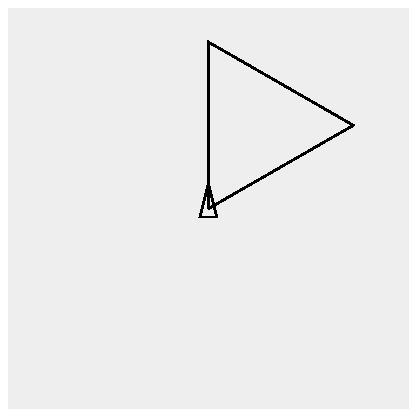
\includegraphics[width=\textwidth]{gfx/2-related-turtle-triangle.pdf}
        \caption{Ergebnis des Dreieck}
        \label{fig:related:turtle:triangle:result}
    \end{subfigure}\hfill
    \begin{subfigure}[b]{0.3\textwidth}
        \includegraphics[width=\textwidth]{gfx/2-related-turtle-house.pdf}
        \caption{Ergebnis des Haus}
        \label{fig:related:turtle:house:result}
    \end{subfigure}
    \caption{Zeichnen eines Hauses in LOGO}
    \label{fig:related:turtle:square}
\end{figure}

%************************************************
% Karel the Robot
%************************************************
\section{Karel the Robot}
\label{sec:related:karel}

Pattis geht mit \textit{Karel the Robot} einen ähnlichen Weg wie die Turtle Grafiken. Aber statt einer Schildkröte wird der Roboter Karel über das Spielfeld bewegt. Karel bewegt sich nicht frei, sondern auf einem Netz von horizontalen (Avenue) und vertikalen Straßen (Street) auf denen sich Wände (Wall) befinden können und den direkten Weg blockieren. Karel bewegt sich immer von Kreuzung zu Kreuzung (Corner). Außerdem können Gegenstände -- sogenannte Beeper -- auf Kreuzungen platziert sein. Diese können von Karel aufgenommen, bewegt und abgesetzt werden. Einige Aufgaben beinhalten das Aufsammeln oder Ablegen von Mustern aus Gegenständen~\cite[1-3]{pattis1981}.

\begin{figure}[h]
    \centering
    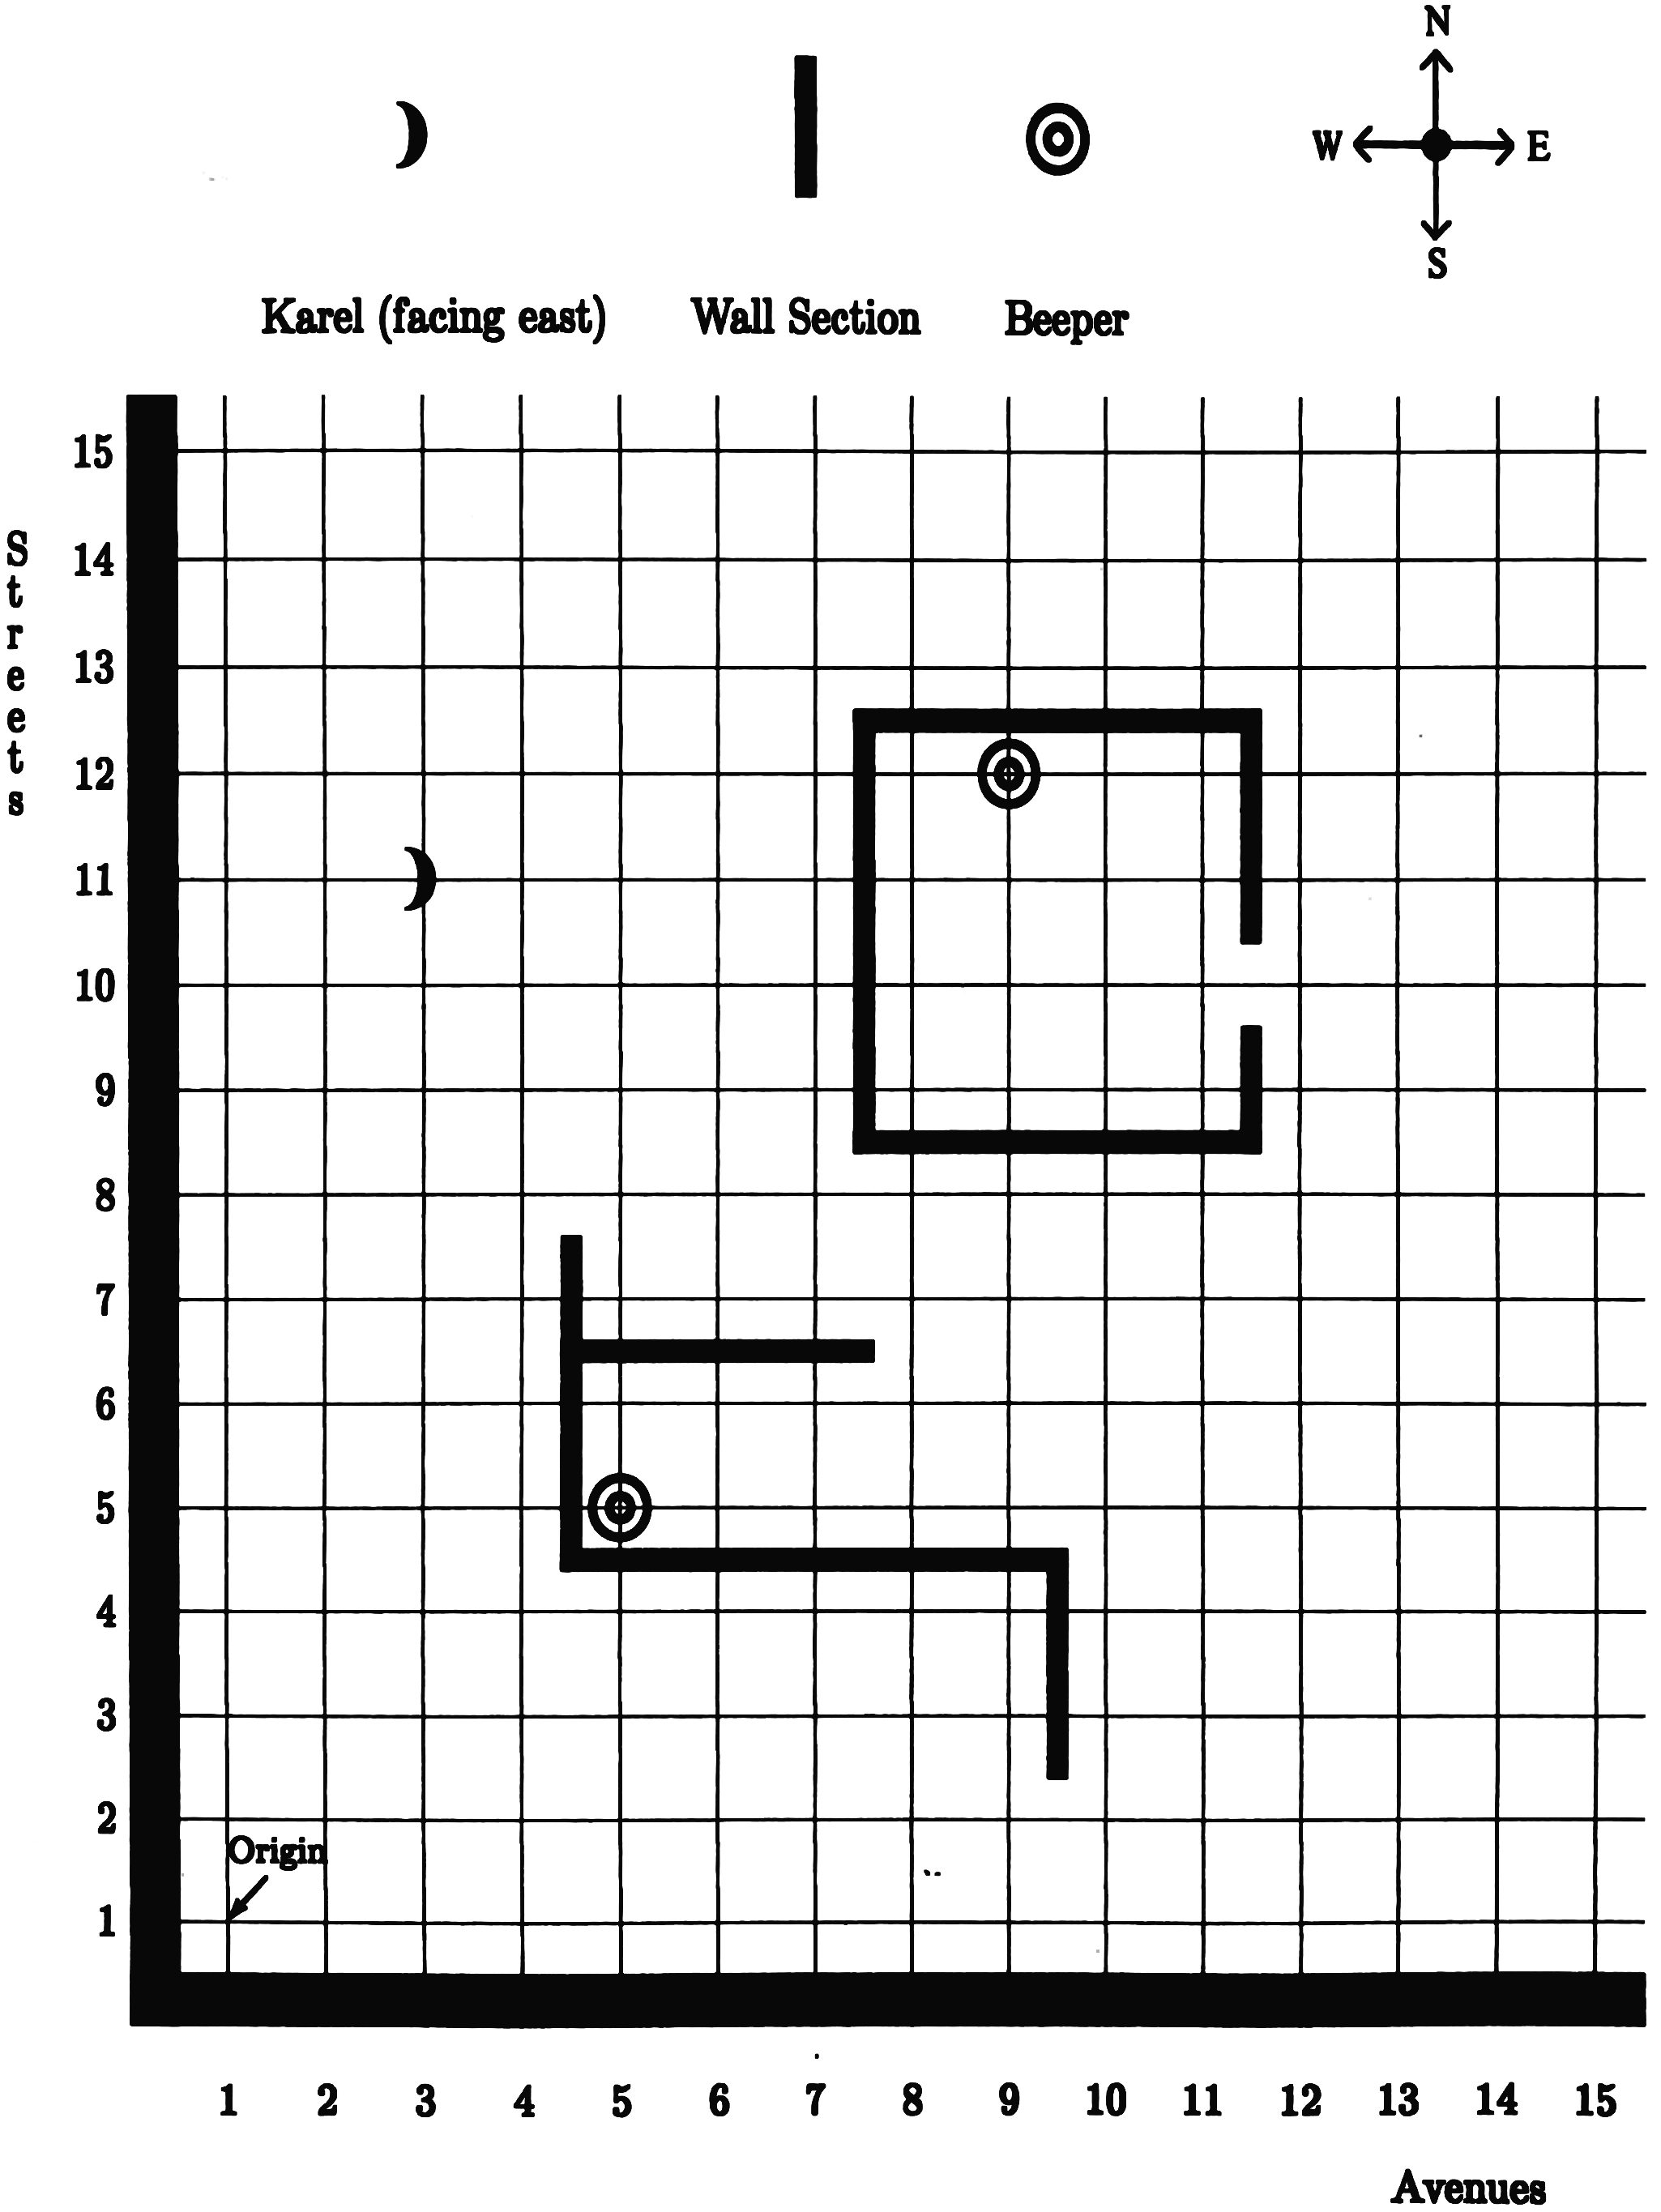
\includegraphics[width=0.5\textwidth]{gfx/2-related-karel.png}
    \caption{Die Struktur von Karels Welt aus~\cite[3]{pattis1981}}
    \label{fig:related:karel}
\end{figure}

%************************************************
% Kara
%************************************************
\section{Kara}
\label{sec:related:kara}

Kara weicht in seiner ursprünglichen Version von den vorhergenannten Programmen ab, indem auf getippte Programmierbefehle zugunsten einer grafischen Oberfläche verzichtet wird. Kara setzt hier auf das Konzept der endlichen Automaten. Reichert et al. beschreiben Kara wie folgt:

\begin{quote}
    "Kara ist eine Mini-Umgebung basierend auf der Idee der endlichen Automaten. Kara, der Marienkäfer, lebt in einer einfachen grafischen Welt auf dem Bildschirm. Der Marienkäfer kann programmiert werden, um in seiner Welt verschiedene Aufgaben zu erledigen. Kleeblätter sammeln, einer Spur von Kleeblättern folgen oder Labyrinthe durchqueren sind einige Beispiele. Die Programme werden grafisch mit der Maus als endliche Automaten erstellt."~\cite[28]{reichert2004}
\end{quote}

Neben der ursprünglichen Idee von Kara mit endlichen Automaten, gibt es weitere Versionen, die den Übergang zu realen Programmiersprachen erleichtern sollen \cite{kara2017}. So lässt sich der Marienkäfer in der bekannten Welt auch mit Java, JavaScript, Python oder Ruby steuern. Durch die Konstrukte die diese Sprachen mitbringen in Verbindung mit den speziellen Methoden, die die Kara-Umgebung zur Verfügung stellt, sind nun auch kompliziertere Programme möglich.

Auch bei Kara gibt es kein durch das Programm definiertes und überprüfbares Spielziel. Es kann eine Aufgabenstellung definiert werden, die zu erfüllen ist, die Kontrolle obliegt allerdings dem Nutzer selbst oder dem Aufgabensteller.

\begin{figure}[h]
    \begin{subfigure}[b]{0.5\textwidth}
        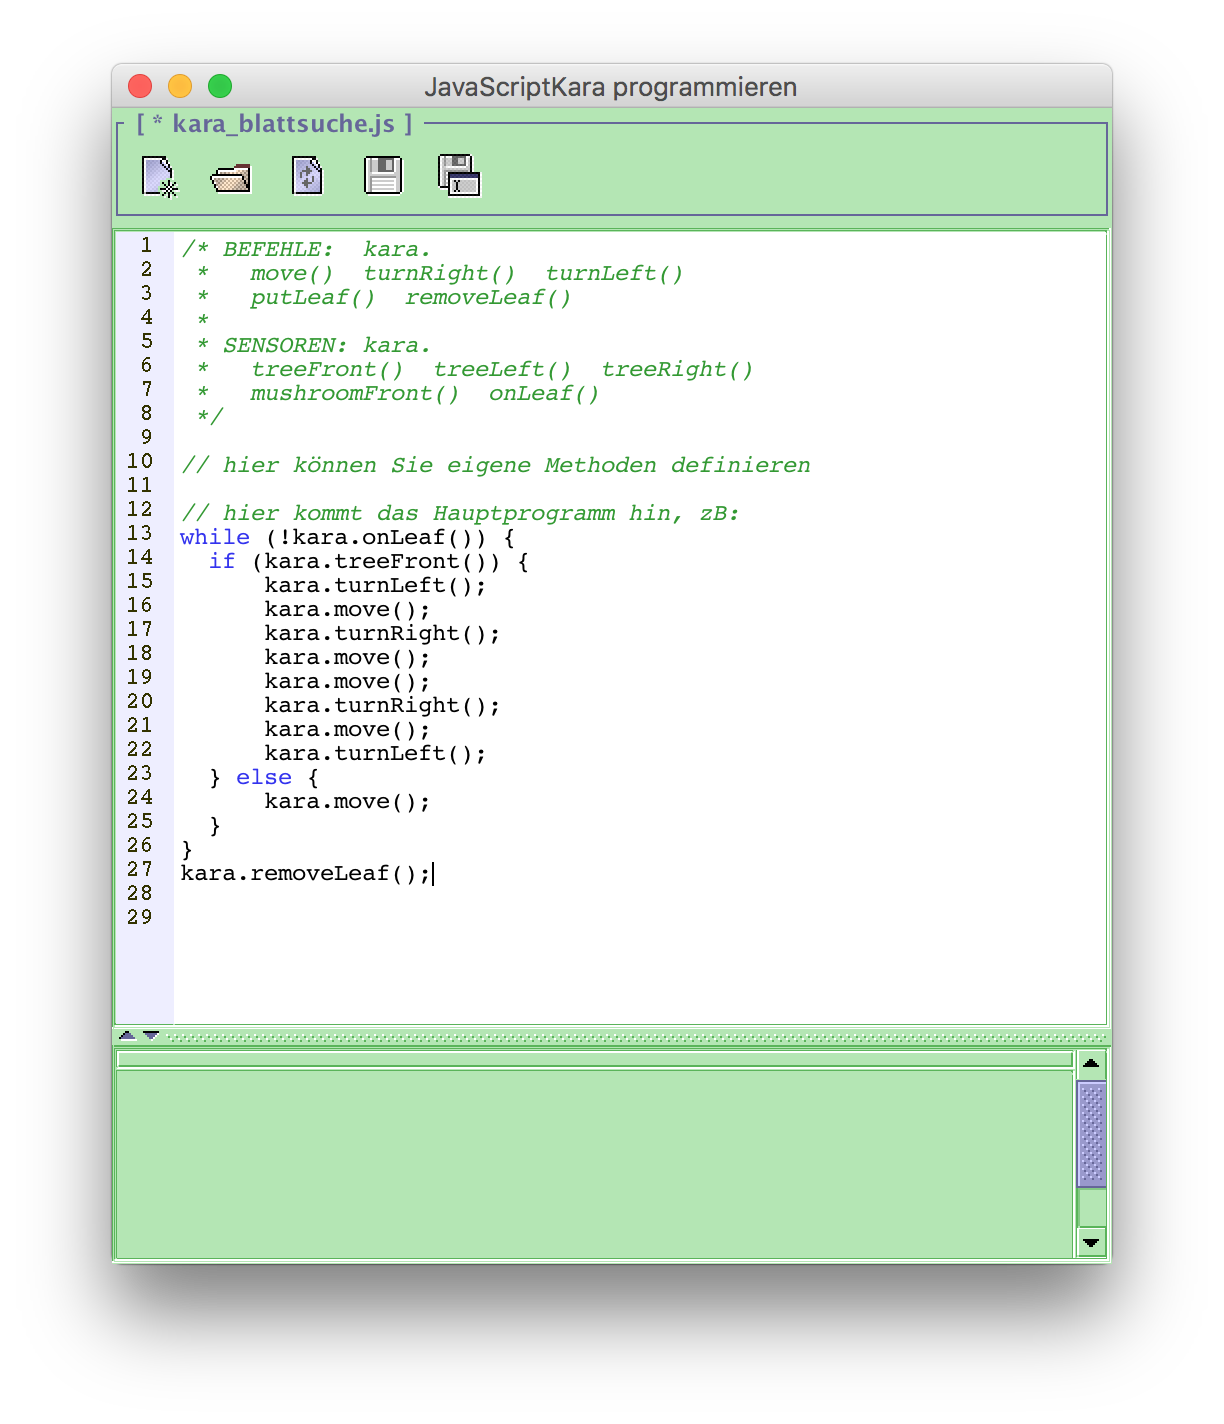
\includegraphics[width=\textwidth]{gfx/2-related-kara-code.png}
        \caption{Suchen eines Blattes in einem Wald}
        \label{fig:related:kara:code}
    \end{subfigure}
    \begin{subfigure}[b]{0.5\textwidth}
        \includegraphics[width=\textwidth]{gfx/2-related-kara-world.png}
        \caption{Kara-Welt}
        \label{fig:related:kara:world}
    \end{subfigure}
    \caption{Bildschirmfoto aus der JavaScriptKara-Anwendung}
    \label{fig:related:kara}
\end{figure}

%************************************************
% Lightbot
%************************************************
\section{Lightbot}
\label{sec:related:lightbot}

Danny Yaroslavski, der Hauptentwickler von Lightbot beschreibt in einem PDF-Dokument sein Programm als ein Denkspiel, welches seine Mechaniken die Konzepten des Programmierens abbildet. Das Ziel von Lightbot ist es, in jedem Level einen Roboter dazu zu bringen, alle blauen Kacheln zu beleuchten. Dazu muss der Roboter mit einer Reihe von Anweisungen "programmiert" werden~\cite{yaroslavski2014}.

Lightbot kommt dabei gänzlich ohne klassische geschriebene Programmieranweisungen aus. Stattdessen werden quadratische Bausteine von einer Toolbox in dafür vorgesehene Bereiche gezogen. Jeder Baustein deutet mit einem Icon den dahinterliegenden Befehl an. Prozeduren müssen verwendet werden, wenn im Bereich für das Hauptprogramm nicht ausreichend Platz vorhanden ist. Für jede Prozedur ist ein zusätzlicher Bereich vorgegeben, der mit einem entsprechenden Baustein aufgerufen werden kann. Neben atomaren Befehlen zum Vorwärtsgehen, Links- und Rechtsdrehen, Springen und Lich An- und Ausschalten, sind mit Lightbot Schleifen lediglich durch rekursive Aufrufe der Prozeduren möglich. Eine Abbruchbedingung kann nicht definiert werden. Auch auf Variablen und Verzweigungen wird verzichtet. Das bedeutet auch, dass der Roboter über keine Sensoren verfügt und blind durch seine Miniwelt läuft. Abbildung~\ref{fig:related:lightbot:screenshot} zeigt ein Bildschirmfoto aus der Lightbot App für iOS\footnote{\url{https://itunes.apple.com/de/app/lightbot-code-hour/id873943739?mt=8}}.

Die Level in der App sind in drei Gruppen aufgeteilt. Im ersten Bereich "Basics" werden die atomaren Befehle eingeführt. Dabei erhöht sich der Schwierigkeitsgrad im Laufe der 8 Level. Im zweiten Bereich "Procedures" werden dann Prozeduren eingeführt und im dritten Teil "Loops" können die Level nur durch den geschickten Einsatz von Rekursion gelöst werden.

Im Gegensatz du den bisher beschriebenen Programmen, gibt es bei Lightbot ein klares Ziel, welches durch das Level definiert ist. Es müssen immer alle Lichter eingeschaltet werden. Sobald dies geschehen ist, ist das Level gelöst und das nächste Level wird freigeschaltet. So ist mit Lightbot auch ein unbeaufsichtigtes Lernen möglich. Die Lösung der Aufgabenstellung muss nicht manuell geprüft werden. Das Programm weißt dadurch eher die Merkmale eines Spiels auf.

\begin{figure}[h]
    \centering
    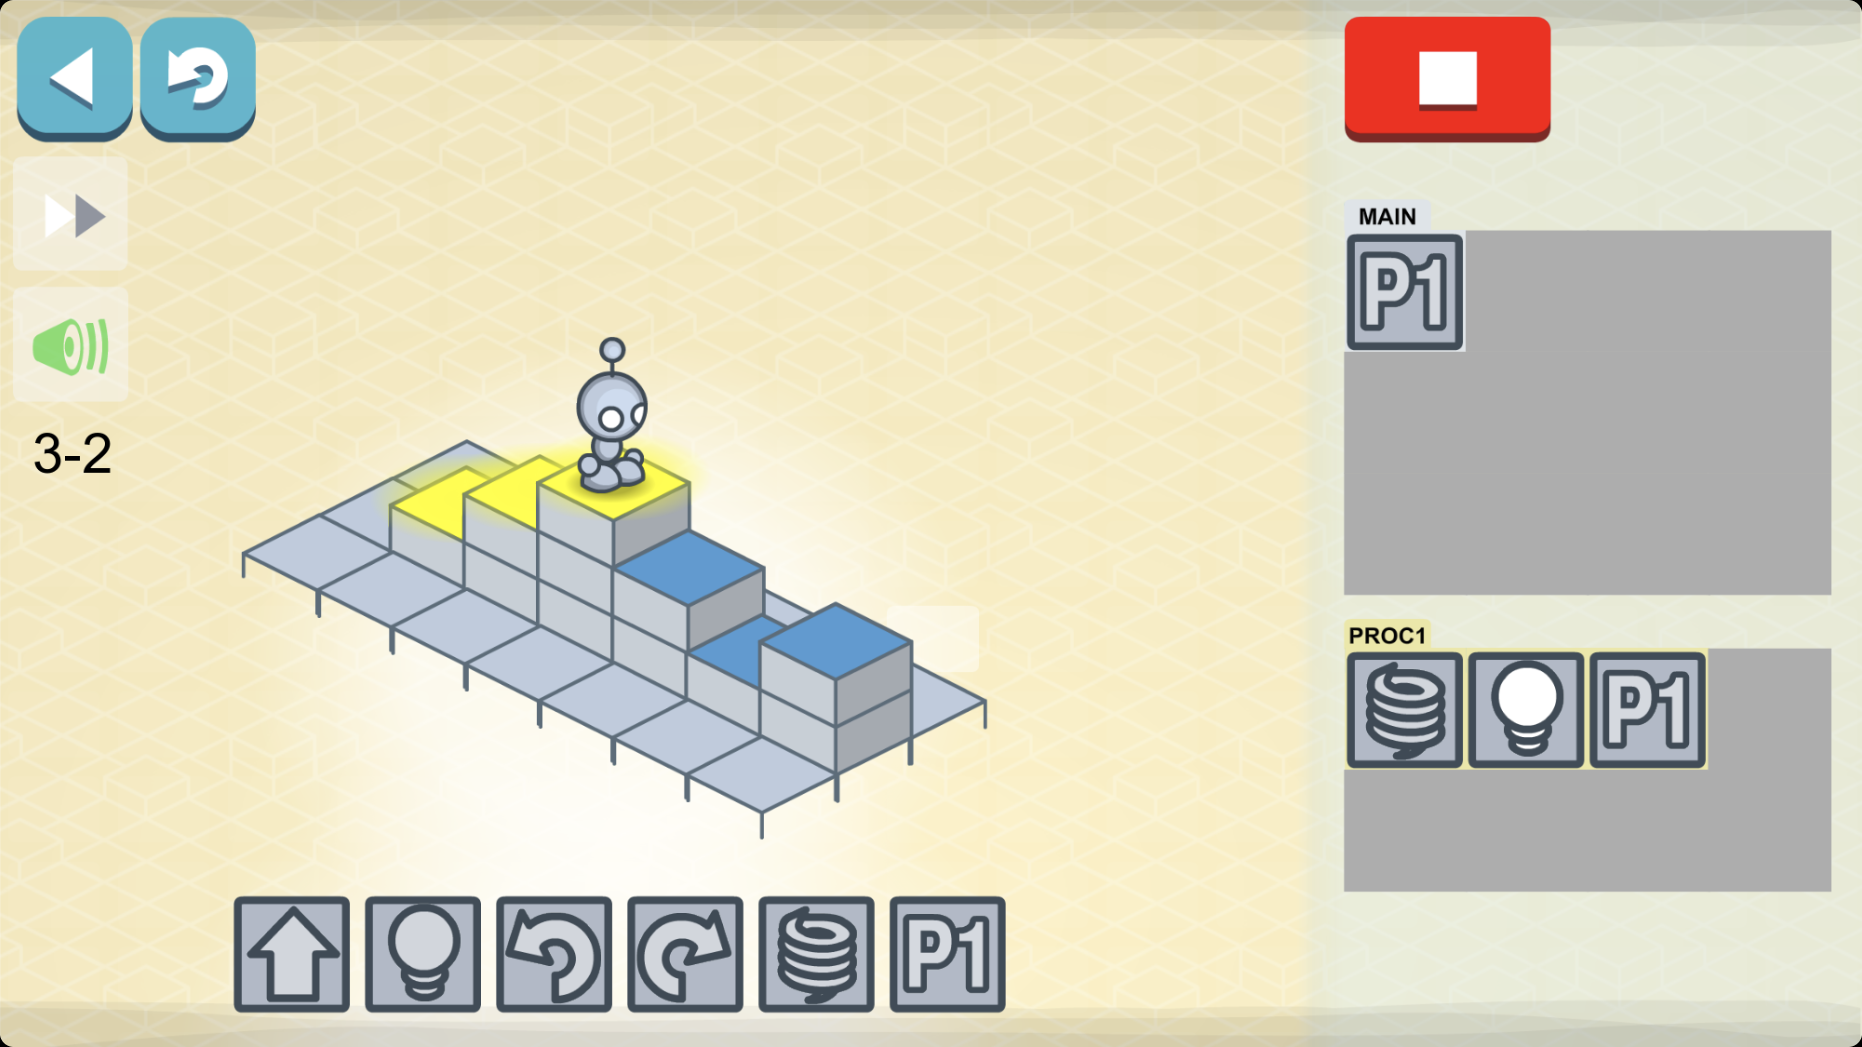
\includegraphics[width=0.8\textwidth]{gfx/2-related-lightbot-screenshot.png}
    \caption{Bildschirmfoto aus der Lightbot App für iOS}
    \label{fig:related:lightbot:screenshot}
\end{figure}
 % INCLUDE: related work
%************************************************
% Anforderungsanalyse
%************************************************
\chapter{Anforderungsanalyse}
\label{sec:requirements}

Aufgabe der Abschlussarbeit ist die Integration eines Tools zum spielerischen Erlernen von Programmierfähigkeiten in die von Marcus Riemer entwickelte Lehr-Entwicklungsumgebung BlattWerkzeug \tref{sec:requirements:existing} sein. Als Vorbilder dieser Anwendung dienen dabei Kara \tref{sec:related:kara} und Lightbot \tref{sec:related:lightbot}. Im Folgenden sind die Anforderungen an dieses Programm näher beschrieben.

%************************************************
% Vorhandenes Projekt
%************************************************
\section{Vorhandenes Projekt}
\label{sec:requirements:existing}

Marcus Riemer hat im Rahmen seiner Master-Thesis an der Fachhochschule Wedel die Lehr-Entwicklungsumgebung BlattWerkzeug entwickelt, die sich an Kinder und Jugendliche richtet. Mit BlattWerkzeug lassen sich gestützt durch Drag \& Drop-Editoren für beliebige SQLite-Datenbanken Abfragen formulieren und Oberflächen entwickeln~\cite[2]{riemer2016}.

\subsection{Aufbau}

\subsubsection{Server}

Der Server ist auf Basis von Ruby mit Sinatra gebaut. Er dient hauptsächlich der Speicherung und Auslieferung von Daten. Kommuniziert wird primär über eine REST-artige JSON-Schnittstelle~\cite[94]{riemer2016}.

Die für diese Arbeit entwickelte Software baut jedoch lediglich auf dem Client von BlattWerkzeug auf und hat mit der serverseitigen Anwendung keine direkten Berührungspunkte.

\subsubsection{Client}

Der Client wurde als eine Single-Page Application mit rein clientseitiger Visualisierung aufgebaut, die weitestgehend auf Roundtrips zum Server verzichtet~\cite[94-95]{riemer2016}. Programmiert wurde sie auf Basis von Angular 2 in TypeScript, wobei der aktuelle Stand inzwischen auf eine höhere Angular-Version setzt.

Durch die direkte Einbindung des im Rahmen dieser Arbeit erstellten Programms, ist die Implementierung in Angular und TypeScript fest vorgegeben.

\subsection{Drag \& Drop-Editor}

Besonders hervorgehoben werden soll an dieser Stelle der Drag \& Drop-Editor von BlattWerkzeug. Auch wenn er nicht direkt Teil dieser Arbeit ist, spielt er doch eine entscheidende Rolle, da über ihn der Großteil der Interaktion abläuft. Programmcode wird nicht getippt sondern aus unterschiedlichen Bausteinen mit der Maus zusammengesetzt.

\begin{quote}
    "So nutzt auch BlattWerkzeug einen Drag \& Drop-Editor um Syntaxfehler von vornherein auszuschließen und kontextsensitiv mögliche Operationen hervorzuheben."~\cite[6]{riemer2016}
\end{quote}

Die Bausteine des Drag \& Drop-Editor und deren Kombinationsmöglichkeiten werden durch die Grammatik festgelegt, die in \treft{sec:requirements:program} näher beschrieben wird. Ergebnis des Drag \& Drop-Editor ist nach dem Bearbeiten durch den Nutzer dann ein Syntaxbaum, der alle Operationen enthält und vom Programm weiterverarbeitet werden kann. \figreft{fig:requirements:existing:draganddrop} zeigt ein Bildschirmfoto des Drag \& Drop-Editor mit einem vollständigen Programm.

\begin{figure}[h]
    \centering
    \includegraphics[width=0.8\textwidth]{gfx/3-requirements-existing-draganddrop.png}
    \caption{Bildschirmfoto des Drag \& Drop-Editor in BlattWerkzeug}
    \label{fig:requirements:existing:draganddrop}
\end{figure}

%************************************************
% Zielgruppe
%************************************************
\section{Zielgruppe}
\label{sec:requirements:target}

Die Zielgruppe wird zum Teil natürlich auch über die Zielgruppe von BlattWerkzeug definiert, wobei sie im Folgenden noch etwa spezieller formuliert und erweitert werden soll.

BlattWerkzeug definiert die Zielgruppe auf Schüler und Schülerinnen ab der Mittelstufe mit grundlegenden PC-Anwenderkenntnissen. Kenntnisse über den Umgang mit Tabellenkalkulationsprogrammen werden nicht als zwingende Voraussetzung, aber als eine sinnvolle Vorstufe, um die Strukturierungsmöglichkeiten von Datenbeständen zu verstehen, angesehen. Für die Entwicklung von Oberflächen werden grundlegende Vorstellungen über die Funktionsweise und Parameter einiger Bedienelemente benötigt. Außerdem wird das Wissen über einzelne englische Vokabeln vorrausgesetzt~\cite[22-23]{riemer2016}.

Schüler grundlegenden PC-Anwenderkenntnissen sollten zur Bedienung des Tools vorhanden sein. Dazu gehört das starten und Bedienen eines Webbrowsers, was bei den meisten Schülern allerdings vorrausgesetzt werden können sollte. Kenntnisse über den Umgang mit Tabellenkalkulationsprogrammen und Vorstellungen über die Funktionsweise und Parameter einiger Bedienelemente ist für die Benutzung ebenfalls nicht notwendig. Schüler, noch nie mit dem Thema Programmierung in Berührung gekommen sind, sollten bei den ersten Schritten von einer Lehrkraft begleitet werden. Nachdem erste Erfahrungen gesammelt wurden, sollten Schüler dann auch selbstständig in der Lage sein neue Möglichkeiten selbst zu entdecken und neue Aufgaben selbstständig zu lösen. Eine Begleitung in Form einer Schritt für Schritt Anleitung durch die Software ist zunächst nicht geplant.

Außerdem sollen auch Lehrer in die Zielgruppe mit aufgenommen werden, denen die Möglichkeit gegeben werden soll Welten und damit Aufgaben für Ihre Schüler zu erstellen und vorzubereiten \tref{sec:requirements:world} und ihre Schüler bei der Lösung der Aufgaben zu unterstützen.

% \TODO{Evtl. grafische Darstellung der Akteure}

%************************************************
% Spielerisches Lernen
%************************************************
\section{Spielerisches Lernen}

Die im Rahmen dieser Arbeit entwickelte Software soll Lehrer dabei unterstützen ihren Schülern die Grundlagen des Programmierens zu vermittelt. Dies soll spielerisch geschehen. Prensky führt in seinem Buch \textit{Digital Game-Based Learning} drei Gründe an warum digitales spielerisches Lernen funktioniert~\cite[147]{prensky2007}:

\begin{enumerate}
    \item Der erste ist das zusätzliche Engagement, das dadurch entsteht, dass das Lernen in einen Spielkontext gebracht wird. Dies kann beträchtlich sein, besonders wenn Menschen nicht lernen wollen.
    \item Der zweite ist der interaktive Lernprozess. Dier kann und sollte abhängig von den Lernzielen viele verschiedene Formen annehmen.
    \item Der dritte ist die Art und Weise, wie die Zwei im Gesamtpaket zusammengefügt werden. Es gibt viele Möglichkeiten, dies zu tun, und die beste Lösung ist sehr kontextabhängig.
\end{enumerate}

Desweiteren hängt der Lernerfolg auch immer stark davon ab, wie Spiele vom Lehrer letztendlich eingesetzt werden, aber auch der Stil des Spieles spielt eine Rollte. Damit Spiele -- Lerspiele im speziellen -- Spaß bringen, müssen sie einige Anforderungen erfüllen. Malone stellt in seinem Artikel \textit{What Makes Computer Games Fun?} eine Checkliste auf, die sich in drei Kategorien gliedert und unter anderem die folgenden Fragen enthält~\cite[49]{malone1981}:

\begin{itemize}
    \item \emph{Herausforderung}: Hat das Spiel ein Ziel? Hat das Spiel einen variablen Schwierigkeitsgrad? Verfügt die Aktivität über mehrere Ziele, z. B. Zählen von Punkten oder schnellere Reaktionen? Enhält das Programm Zufall? Enthält das Programm versteckte Informationen die selektiv aufgedeckt werden?
    \item \emph{Fantasie}: Enthält das Programm eine emotional ansprechende Fantasie? Hängt die Fantasie instinktiv mit der in der Aktivität erlernten Fähigkeit zusammen? Ist die Phantasie eine nützliche Metapher?
    \item \emph{Neugierde}: Gibt es audio- und visuelle Effekte, um die Neugier der Sinne zu stimulieren? Gibt es Elemente, die die kognitive Neugier wie Überraschungen oder konstruktives Feedback stimulieren?
\end{itemize}

Auch wenn nicht alle durch das entwickelte Spiel erfüllt werden können, sollte es doch das Ziel sein so vielen Anforderungen wie möglich gerecht zu werden, um die Aktivität für den Schüler so interessant wie möglich zu gestalten.

%************************************************
% Welt
%************************************************
\section{Welt}
\label{sec:requirements:world}

Die im vorherigen Abschnitt beschriebenen Anforderungen lassen sich sehr gut mit den Lerzielen vereinbaren. Ein Objekt wird mit programmierten Befehlen durch eine virtuelle Welt geführt. Der Spieler löst so eine Art Puzzelrätsel.

\subsection{Handlungsgerüst}
\label{sec:requirements:world:metaphor}

Um nachfolgend die Definition der Anforderungen zu erleichern, wird bereits an dieser Stelle die Metapher beschrieben. Ziel des Spiels soll es sein mit Hilfe eines Lastwagen, welcher vom Spieler über Programmbefehle steuerbar ist \tref{sec:requirements:program}, über ein Netz von Straßen, verschiedenfarbige Container an ihre vorgesehenen Ziele zu bringen. Dabei ist die Ladefläche des Lastwagen begrenzt, womit unter Umständen mehrfache Fahrten notwendig sind. Zusätzlich kann der Tank des Lastwagen begrenzt sein, wodurch es für die Lehrkraft denkbar wäre eine intelligente Routenführung Teil der Aufgabe zu machen.

Diese Metapher wurde gewählt, da der Transport von Waren in dieser vereinfachten Darstellung jedem bekant sein sollte. Außerdem bietet die Metapher verschiedene Erweiterungsmöglichkeiten und ermöglicht eine schrittweise Erhöhung der Komplexität. So ist z.B. die Einführung von Verkehrsampeln zur Vermittlung des Konzeptes der Verzweigungen möglich.

\subsection{Datenstruktur}
\label{sec:requirements:world:structure}

In Anlehnung an Kara soll die Möglichkeit gegeben werden neue Level, bzw. Aufgaben zu entwerfen. Jede Aufgabe besteht dabei aus einer Welt Wobei sowohl Lehrer, als auch Schüler in der Lage sein sollen neue Welten zu erstellen. Die Funktion richtet sich jedoch primär an die Lehrkraft. In Anlehnung an Lightbot ist das Ziel der Aufgabe jedoch immer dadurch definiert, dass alle Container -- die sich zu Beginn des Level bereits auf der Ladefläche oder an einer beliebigen Straße im Spielfeld befinden können -- an ihr vorgesehenes Ziel gebracht werden.

Es kann davon ausgegangen werden, dass ein Lehrer für das Fach Informatik über Rfahrung in der Bedienung auch von komplexeren Programen verfügt. Daher kann die Umgebung zur Gestaltung der Level eher zweckmäßig sein und setzt keinen Fokus auf eine leichte Bedienung.

Um diese Funktionalität zu ermöglichen, muss für BlattWerkzeug eine Datenstruktur gebaut werden, durch die sich mit dem Drag \& Drop-Editor eine Welt bauen lässt.

%************************************************
% Programm
%************************************************
\section{Programm}
\label{sec:requirements:program}

Die Bewegungsabläufe wie z.B. "geradeaus fahren", "links abbiegen", "rechts abbiegen" oder "warten" werden vom Nutzer mittels des Drag \& Drop-Editor programmiert. Dafür wird eine Minisprache eingeführt, die über einen reduzierten Funktionsumfang verfügt und dadurch den Nutzer behutsam an das Thema heranführen soll und den Nutzer nicht wie Universalsprachen mit einem großen Sprachumfang und der damit verbundennen steileren Lernkurve überfordern sollen. Brusilovsky et al. heben in Ihrem Artikel \textit{Mini-languages: a way to learn programming principles} einige Eigenschaften von Minisprachen als besonders wichtig hervor \cite[73-74]{brusilovsky1997}:

\begin{itemize}
    \item Sowohl Syntax, als auch Semantik der Sprache sollte \emph{einfach} sein.
    \item Die Operationen der Minisprache sollten \emph{sichtbar} sein. Die meisten Operationen, die der Akteur ausführt, sollten sichtbare Änderungen in der auf dem Bildschirm dargestellten Mikrowelt vornehmen.
    \item Die Minisprache sollte für die vorgesehene Kategorie von Studenten \emph{attraktiv} und aussagekräftig sein.
    \item Die Sprache sollte \emph{dialogorientiert} sein. Das Bedeutet, dass die Sprache Befehl für Befehl in einem Navigationsmodus ausgeführt werden kann (Einzelbefehlsausführung) und in einem Programmiermodus (komplexe Programmausführung).
    \item Die Sprache sollte \emph{modular} sein. Sie sollte einen Mechanismus zum Erstellen abstrakter Anweisungen (Prozeduren) enthalten. Alle Verfahren sollten unabhängige Einheiten sein. Eine solche Prozedur kann als neuer Befehl des Akteurs betrachtet werden, der sowohl im Navigations- als auch im Programmiermodus verwendet werden kann.
\end{itemize}

% Brusilovsky et al. nennen in Ihrem Artikel \textit{Mini-languages: a way to learn programming principles} drei Probleme mit Universalsprachen (wie z.B. Java oder C) für die Anwendung zum Lernen, die Minisprachen zu beheben versuchen \cite[67]{brusilovsky1997}:

% \begin{itemize}
%     \item Universalsprachen sind zu groß und zu idiosynkratisch. Die konzeptionelle Basis der Sprache bildet zusammen mit den Hauptprinzipien der Programmierung eine große Menge an Material. Anstatt die Grundprinzipien hervorzuheben, rufen die Sprachen \TODO{evoke secondary notions / sekundäre Begriffe} hervor, die die Feinheiten der jeweiligen Sprache und deren Umsetzung widerspiegeln.
%     \item Universalsprachen fördern nicht das Verständnis ihrer grundlegenden Aktionen und Kontrollstrukturen. Die Sprachen sind nicht visuell und ihre Grundfunktionen werden hinter einer undurchsichtigen Barriere ausgeführt. Wenn der Prozess der Programmausführung verborgen ist, entwickelt der Student ein Input-Output-orientiertes Verständnis. Auf diese Weise behindert das Fehlen von visuellem Feedback die Beherrschung der Sprachsemantik.
%     \item Da sich Universalsprachen an der Zahlen- und Symbolverarbeitung orientieren, sind die ersten möglichen Aufgaben, die beim Unterrichten der Sprache umgesetzt werden können, weit von den Alltagserfahrungen der Schüler entfernt. Die Entwicklung von Anwendungen, die sowohl informativ als auch interessant sind, erfordert das Erlernen einer beträchtlichen Untermenge der Sprache und das Schreiben recht großer Programme.
% \end{itemize}

\subsection{Datenstruktur}
\label{sec:requirements:program:structure}

\TODO{Datenstruktur}

\subsection{Kompilieren / Interpretieren}
\label{sec:requirements:world:compile-interpret}

\TODO{Kompilieren / Interpretieren}

% Wagenknecht und Hielscher beschreiben den Unterschied zwischen Kompilieren und Interpretieren wie folgt:

% \begin{quote}
%     "Programme, die Programme einer Quellsprache in zugehörige Programme einer Zielsprache überführen, nennt man \emph{Compiler}. [...] Statt Anwendungsprogramme aus maschienennahen Instruktionen aufzubauen, verwendet man menschenfreundlichere Sprachelemente [...]. Damit diese Programme von [...] einem Prozessor und dem Betriebsystem verarbeitet werden können, ist eine entsprechende Übersetzung notwendig. [...] \emph{Interpreter} gehen anders vor als Compiler. Das vorgelegte Programm wird nicht vollständig übersetzt, sondern "portionsweise" analysiert, in eine zugehörige Folge von Prozessorintruktionen übertragen und ausgeführt."~\cite[47]{wagenknecht2009}
% \end{quote}

\subsection{Darstellung der Ausführung}
\label{sec:requirements:world:display}

\TODO{Darstellung der Ausführung}
 % INCLUDE: system
%************************************************
% Implementierung
%************************************************
\chapter{Implementierung}
\label{sec:implementation}

\TODO{Implementierung}
 % INCLUDE: concepts
%************************************************
% Fazit
%************************************************
\chapter{Fazit}
\label{sec:conclusion}

\TODO{Fazit}

\section{Erreichte Ziele}
\label{sec:conclusion:archived}

\TODO{Erreichte Ziele}

\section{Nicht erreichte Ziele}
\label{sec:conclusion:open}

\TODO{Nicht erreichte Ziele}

\section{Weitere Entwicklung}
\label{sec:conclusion:future}

\TODO{Weitere Entwicklung}

\TODO{A promising way of further development of mini-language programming environments is to extend them with an intelligent tutoring component and a hypermedia component. \cite{brusilovsky1997}}
 % INCLUDE: conclusion
\cleardoublepage

% --------------------------
% Back matter
% --------------------------
{%
\setstretch{1.1}
\renewcommand{\bibfont}{\normalfont\small}
\setlength{\biblabelsep}{0pt}
\setlength{\bibitemsep}{0.5\baselineskip plus 0.5\baselineskip}
% \printbibliography
\printbibliography[title=Literaturverzeichnis,nottype=online]
\printbibliography[heading=subbibliography,title={Quellen im Internet},type=online,prefixnumbers={@}]
}
\cleardoublepage

% \listoffigures
% \cleardoublepage

% \listoftables
% \cleardoublepage

%************************************************
% Declaration
%************************************************
\pdfbookmark[0]{Eidesstattliche Erklärung}{Eidesstattliche Erklärung}
\chapter*{Eidesstattliche Erklärung}
\label{sec:declaration}
\thispagestyle{empty}

Ich erkläre hiermit an Eides statt, dass ich die vorliegende Arbeit selbstständig und ohne Benutzung anderer als der angegebenen Hilfsmittel angefertigt habe; die aus fremden Quellen direkt oder indirekt übernommenen Gedanken sind als solche kenntlich gemacht. Die Arbeit wurde bisher in ähnlicher Form keiner anderen Prüfungskommission vorgelegt und auch nicht veröffentlicht.

\bigskip
\bigskip
\bigskip
\bigskip

\begin{multicols}{2}
    \raggedright
    \thesisUniversityCity, \thesisDate

    \raggedleft
    \thesisAuthor
\end{multicols}

\cleardoublepage
